% !TEX TS-program = xelatex
% !TEX encoding = UTF-8 Unicode
\documentclass[11pt,a4paper]{article}
\usepackage{amsmath,amssymb}
\usepackage{empheq}
\usepackage[semibold]{ebgaramond}
\usepackage[cmintegrals,cmbraces]{newtxmath}
\usepackage{ebgaramond-maths}
\usepackage{bm}
\usepackage[OMLmathrm, OMLmathsfit, rmdefault=mdugm]{isomath}
\usepackage{tocbibind}
\usepackage{graphicx}
\graphicspath{{./pics/}}
\usepackage{wrapfig}
\usepackage{capt-of}

\makeatletter
  \DeclareSymbolFont{ntxletters}{OML}{ntxmi}{m}{it}
  \SetSymbolFont{ntxletters}{bold}{OML}{ntxmi}{b}{it}
  \re@DeclareMathSymbol{\leftharpoonup}{\mathrel}{ntxletters}{"28}
  \re@DeclareMathSymbol{\leftharpoondown}{\mathrel}{ntxletters}{"29}
  \re@DeclareMathSymbol{\rightharpoonup}{\mathrel}{ntxletters}{"2A}
  \re@DeclareMathSymbol{\rightharpoondown}{\mathrel}{ntxletters}{"2B}
  \re@DeclareMathSymbol{\triangleleft}{\mathbin}{ntxletters}{"2F}
  \re@DeclareMathSymbol{\triangleright}{\mathbin}{ntxletters}{"2E}
  \re@DeclareMathSymbol{\partial}{\mathord}{ntxletters}{"40}
  \re@DeclareMathSymbol{\flat}{\mathord}{ntxletters}{"5B}
  \re@DeclareMathSymbol{\natural}{\mathord}{ntxletters}{"5C}
  \re@DeclareMathSymbol{\star}{\mathbin}{ntxletters}{"3F}
  \re@DeclareMathSymbol{\smile}{\mathrel}{ntxletters}{"5E}
  \re@DeclareMathSymbol{\frown}{\mathrel}{ntxletters}{"5F}
  \re@DeclareMathSymbol{\sharp}{\mathord}{ntxletters}{"5D}
  \re@DeclareMathAccent{\vec}{\mathord}{ntxletters}{"7E}
\makeatother

\usepackage{array}
\usepackage{enumitem}
% to produce a comma between multiple footnotes / https://tex.stackexchange.com/questions/40072/incompatibility-between-footmisc-option-multiple-and-hyperref/62091#62091
\let\oldFootnote\footnote
\newcommand\nextToken\relax
\renewcommand\footnote[1]{%
    \oldFootnote{#1}\futurelet\nextToken\isFootnote}
\newcommand\isFootnote{%
    \ifx\footnote\nextToken\textsuperscript{,}\fi}

\defaultfontfeatures{Ligatures=TeX} % makes this a feature for all selected fonts
\usepackage{esint}
\usepackage{polyglossia}
\setmainlanguage{english}
\usepackage[text={18cm,26cm},centering]{geometry} % 
\usepackage{natbib}
\usepackage{mdframed}
\usepackage{lipsum}
\usepackage[usenames,dvipsnames,svgnames,table]{xcolor}
\usepackage{hyperref}
\usepackage{url}
\usepackage{pdfpages}
\usepackage[export]{adjustbox}

\hypersetup{
  colorlinks,
  citecolor=bleuSU,
  linkcolor=bleuSU
}
\definecolor{bleuSU}{RGB}{26,39,101}

\usepackage[normalem]{ulem}
\makeatletter
\renewcommand*{\uuline}{%
  \bgroup
  \UL@setULdepth
  \markoverwith{%
    \lower\ULdepth\hbox{%
      \kern-.03em%
      \vtop{%
        \hrule width.2em%
        \kern 0.6pt % distance between the two underlines
        \hrule
      }%
      \kern-.03em%
    }%
  }%
  \ULon
}
\makeatother
\setlength{\ULdepth}{-2pt}  % distance from double underline to letter

\usepackage{environ}
\newtoggle{corrige}

\NewEnviron{answer}{%
  \iftoggle{corrige}
    {\begin{mdframed}\textbf{Answer: } \BODY\end{mdframed}}
    {}%
  }

\newcommand{\delS}{\delta S}
\newcommand{\delA}{\delta A}
\newcommand{\delh}{\delta h}
\newcommand{\delt}{\delta t}
\newcommand{\delz}{\delta z}
\newcommand{\delbx}{\delta \matrixsym x}
\newcommand{\lp}{\left(}
\newcommand{\rp}{\right)}
\newcommand{\itA}{\textit A}
\newcommand{\itB}{\textit B}
\newcommand{\dAB}{\mathcal D_{AB}}
\newcommand{\bA}{\matrixsym A}
\newcommand{\bff}{\matrixsym{f}}
\newcommand{\bF}{\matrixsym{F}}
\newcommand{\bj}{\matrixsym{j}}
\newcommand{\bJ}{\matrixsym J}
\newcommand{\bn}{\matrixsym{n}}
\newcommand{\bN}{\matrixsym N}
\newcommand{\bP}{\matrixsym{P}}
\newcommand{\br}{\matrixsym r}
\newcommand{\bt}{\matrixsym t}
\newcommand{\be}{\matrixsym e}
\newcommand{\bu}{\matrixsym u}
\newcommand{\bv}{\matrixsym v}
\newcommand{\bw}{\matrixsym w}
\newcommand{\bx}{\matrixsym x}
\newcommand{\pd}[2]{\frac{\partial #1}{\partial #2}}
\newcommand{\D}[2]{\frac{D #1}{D #2}}
\newcommand{\dd}[2]{\frac{\mathrm d #1}{\mathrm d #2}}
\newcommand{\dA}{\mathrm dA}
\newcommand{\dV}{\mathrm dV}
\newcommand{\dS}{\mathrm dS}
\newcommand{\prg}[1]{\paragraph{$\rhd$ #1}}
\newcommand{\alphaijkl}{\alpha_{ijkl}}
\newcommand{\Aijkl}{A_{ijkl}}
\newcommand{\delij}{\delta_{ij}}
\newcommand{\sigij}{\sigma_{ij}}
\newcommand{\sigji}{\sigma_{ji}}
\newcommand{\sigxy}{\sigma_{xy}}
\newcommand{\matL}{\mathcal L}
\newcommand{\matO}{\mathcal O}
\newcommand{\matS}{\mathcal S}
\newcommand{\kij}{k_{ij}}
\newcommand{\tensor}[1]{\smash{\uuline{#1}{}}}
\setlength{\parindent}{0pt} % remove indent

\setlist[enumerate]{topsep=0pt,itemsep=-1ex,partopsep=1ex,parsep=1ex}

\begin{document}
\setlength{\unitlength}{1cm}
\noindent
\parbox{\textwidth}{
\textsc{
Sorbonne Université  
\hfill
Year 2022-2023
}
}
\parbox{\textwidth}{
\textsc{
Faculté des Sciences
\hfill
Physics of Fluids \& Nonlinear Physics
}
}

\begin{center}
\Large
\textbf{Hydrodynamics} \\ 
\textsl{Tutorial 3: viscous flows} \\[1ex]
\end{center}

\section{Taylor' scraper (1962)}
\begin{figure}[ht]
    \centering
    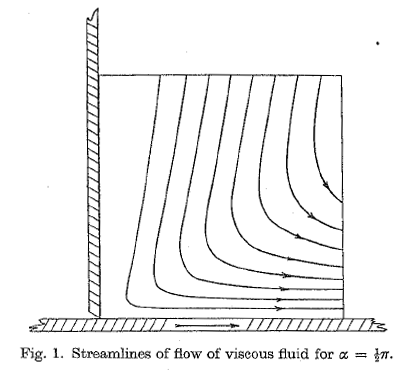
\includegraphics{p411_taylor.png}
    \caption{\textbf{Forced flow in a corner of angle $\alpha$.} Streamlines of the viscous flow induced by the displacement of the bottom plate at velocity $U$ (here $\alpha = \frac{\pi}{2}$).}
    \label{fig:scraper}
\end{figure}
\begin{enumerate}
\item Write down the equations and boundary conditions describing this problem in native variables (pressure/velocity).
\item We look for a solution to this flow by introducing the streamfunction $\psi$ such that $\boldsymbol u = -\nabla \times \big( \psi(r,\theta)\boldsymbol e_z\big)$. Show that the Stokes equations can be reduced to:
\begin{equation}
\nabla^4 \psi = 0
\end{equation}
\item Show that the boundary conditions for $\psi$ are (supposing that the plate advances at velocity $-U$):
 \begin{subequations}
\begin{empheq}[left=\empheqlbrace]{align}
\frac{\partial \psi}{\partial r} = 0 \quad &\text{et} \quad \frac{1}{r}\frac{\partial \psi}{\partial \theta} = U  &&\text{en } \theta = 0 \\[1em]
\frac{\partial \psi}{\partial r} = 0 \quad &\text{et} \quad \frac{1}{r}\frac{\partial \psi}{\partial \theta} = 0  &&\text{en } \theta = \alpha
\end{empheq}
\end{subequations}
\item We look for a solution $\psi$ under the following form:
\begin{equation}
\psi(r,\theta) = r f(\theta)
\end{equation}
Justify this choice.
\item Introducing the differential operator $\mathcal D = \frac{\mathrm d^2}{\mathrm d \theta^2} + \mathcal I$, where $\mathcal I$ is the identity operator, show that:
\begin{equation}
\mathcal D^2 f = 0.
\end{equation}
Deduce the general form of $f(\theta)$:
\begin{equation}
f(\theta) = A \sin \theta + B \cos \theta + C \theta \sin \theta + D \theta \cos \theta
\end{equation}
\item Explicit the boundary conditions for $f(\theta)$.
\item By application of these boundary conditions, show:
\begin{equation}
\big( A,B,C,D \big) = \big(\alpha^2, 0, -\alpha + \sin \alpha \cos \alpha, -\sin^2 \alpha \big) \times \frac{U}{\alpha^2 - \sin^2 \alpha}.
\end{equation}
\item Represent with Python these streamlines for $\alpha = \frac{\pi}{4}, \frac{\pi}{2}, \frac{2\pi}{4}, \pi$.
\item Estimate the order of magnitude the neglected acceleration term in the Stokes approximation as a function of $\rho$, $U$ et $r$. Evaluate as well the order of magnitude of the viscous force. Deduce a region of validity for this approximation as a function of $\mu$, $\rho$ et $U$.
\item Retrieve the expression for the normal stress exerted on the scraper found by Talor.
\item Discuss his conclusion on the way painters use their scraper to clean their palette.
\end{enumerate}

\section{Flow motion induced by microorganisms}
\begin{figure}[ht]
    \centering
    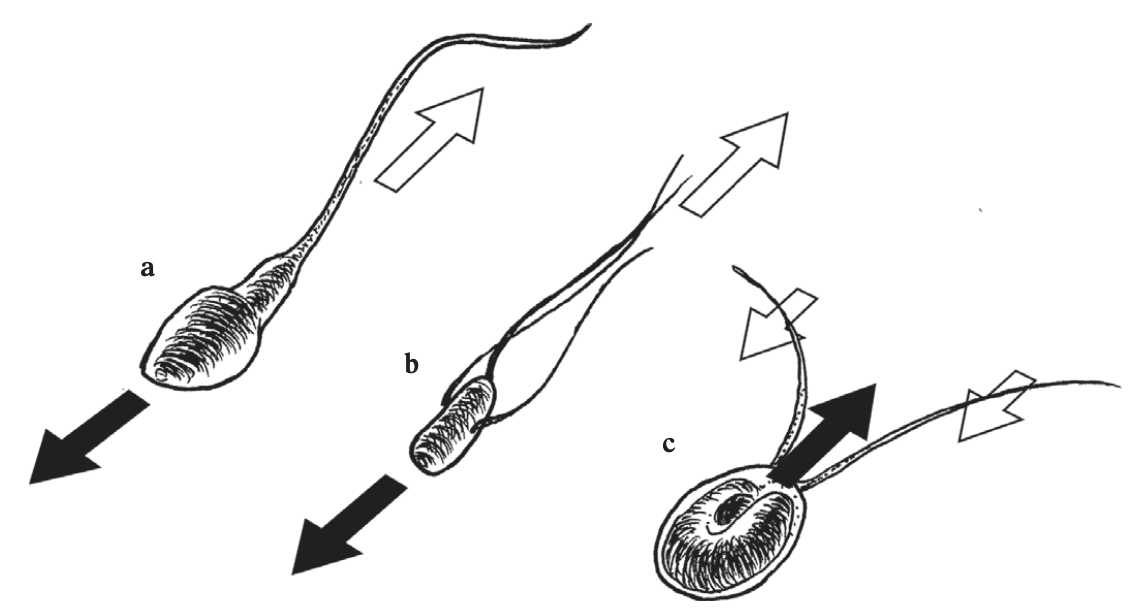
\includegraphics[width=8cm]{microorganisms.png}
    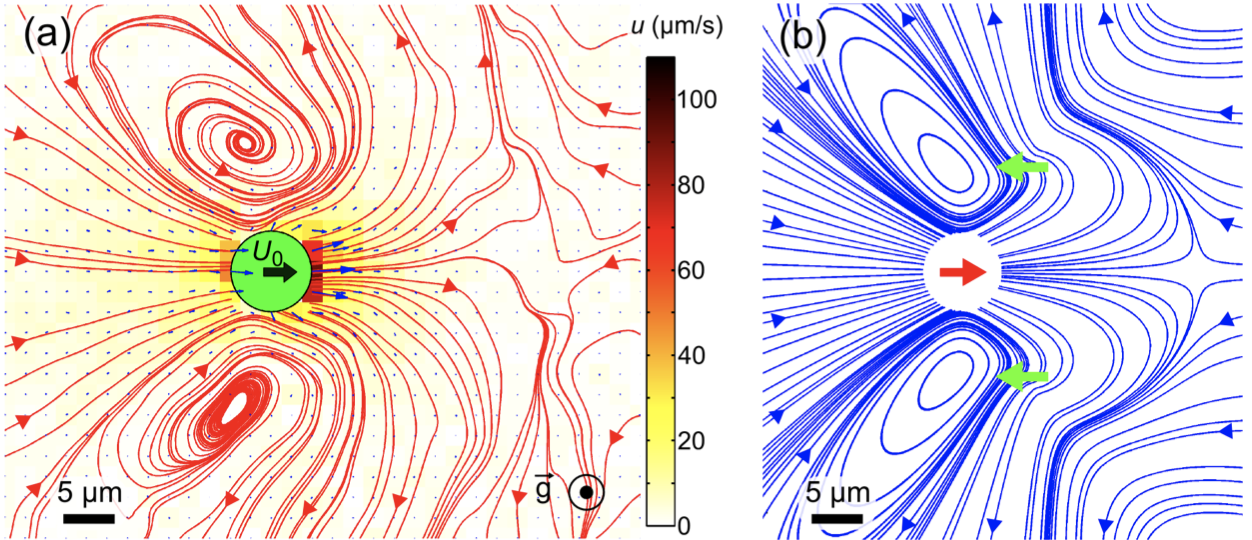
\includegraphics[width=8cm]{drescher.png}
    \caption{\textbf{Swimming microorganisms}. Left: several microorganisms swimming: spermatozoon, bacterium, biflagellated alga (Lauga, 2020). Right: the flow motion measured around a swimming alga (red lines) can be well approximated with a superposition of Stokeslets (Drescher \textit{et al.}, 2010).}
    \label{fig:microorg}
\end{figure}
\begin{enumerate}
\item Represent with Python the streamlines around a single Stokeslet.
\item Using the superposition principle, try to reproduce the flow pattern around a swimming biflagellated alga (hint: consider three Stokeslets as indicated in the figure, of net zero force).
\end{enumerate}
\section*{Appendix: differential operators in cylindrical coordinates}
\noindent Let $f(r,\theta,z)$ be a scalar function of space and $\boldsymbol{u}(r,\theta,z) = (u_r(r,\theta,z), u_\theta(r,\theta,z), u_z(r,\theta,z))$ a vector field. We define:
\begin{equation*}
\nabla f = \left(
\begin{array}{c}
\displaystyle\frac{\partial f}{\partial r}\\[1em]
\displaystyle\frac{1}{r}\frac{\partial f}{\partial \theta}\\[1em]
\displaystyle\frac{\partial f}{\partial z}
\end{array}
\right), 
\quad \nabla \cdot \boldsymbol{u} = \frac{1}{r} \frac{\partial}{\partial r}\bigg( r u_r\bigg) + \frac{1}{r} \frac{\partial u_\theta}{\partial \theta} + \frac{\partial u_z}{\partial z},
\quad \Delta f = \frac{1}{r} \frac{\partial}{\partial r}\bigg( r \frac{\partial f}{\partial r}\bigg) + \frac{1}{r^2} \frac{\partial^2 f}{\partial \theta^2} + \frac{\partial^2 f}{\partial z^2}
\end{equation*}
%\includepdf[pages={1-5}]{Taylor_viscous_fluid_deposition.pdf}
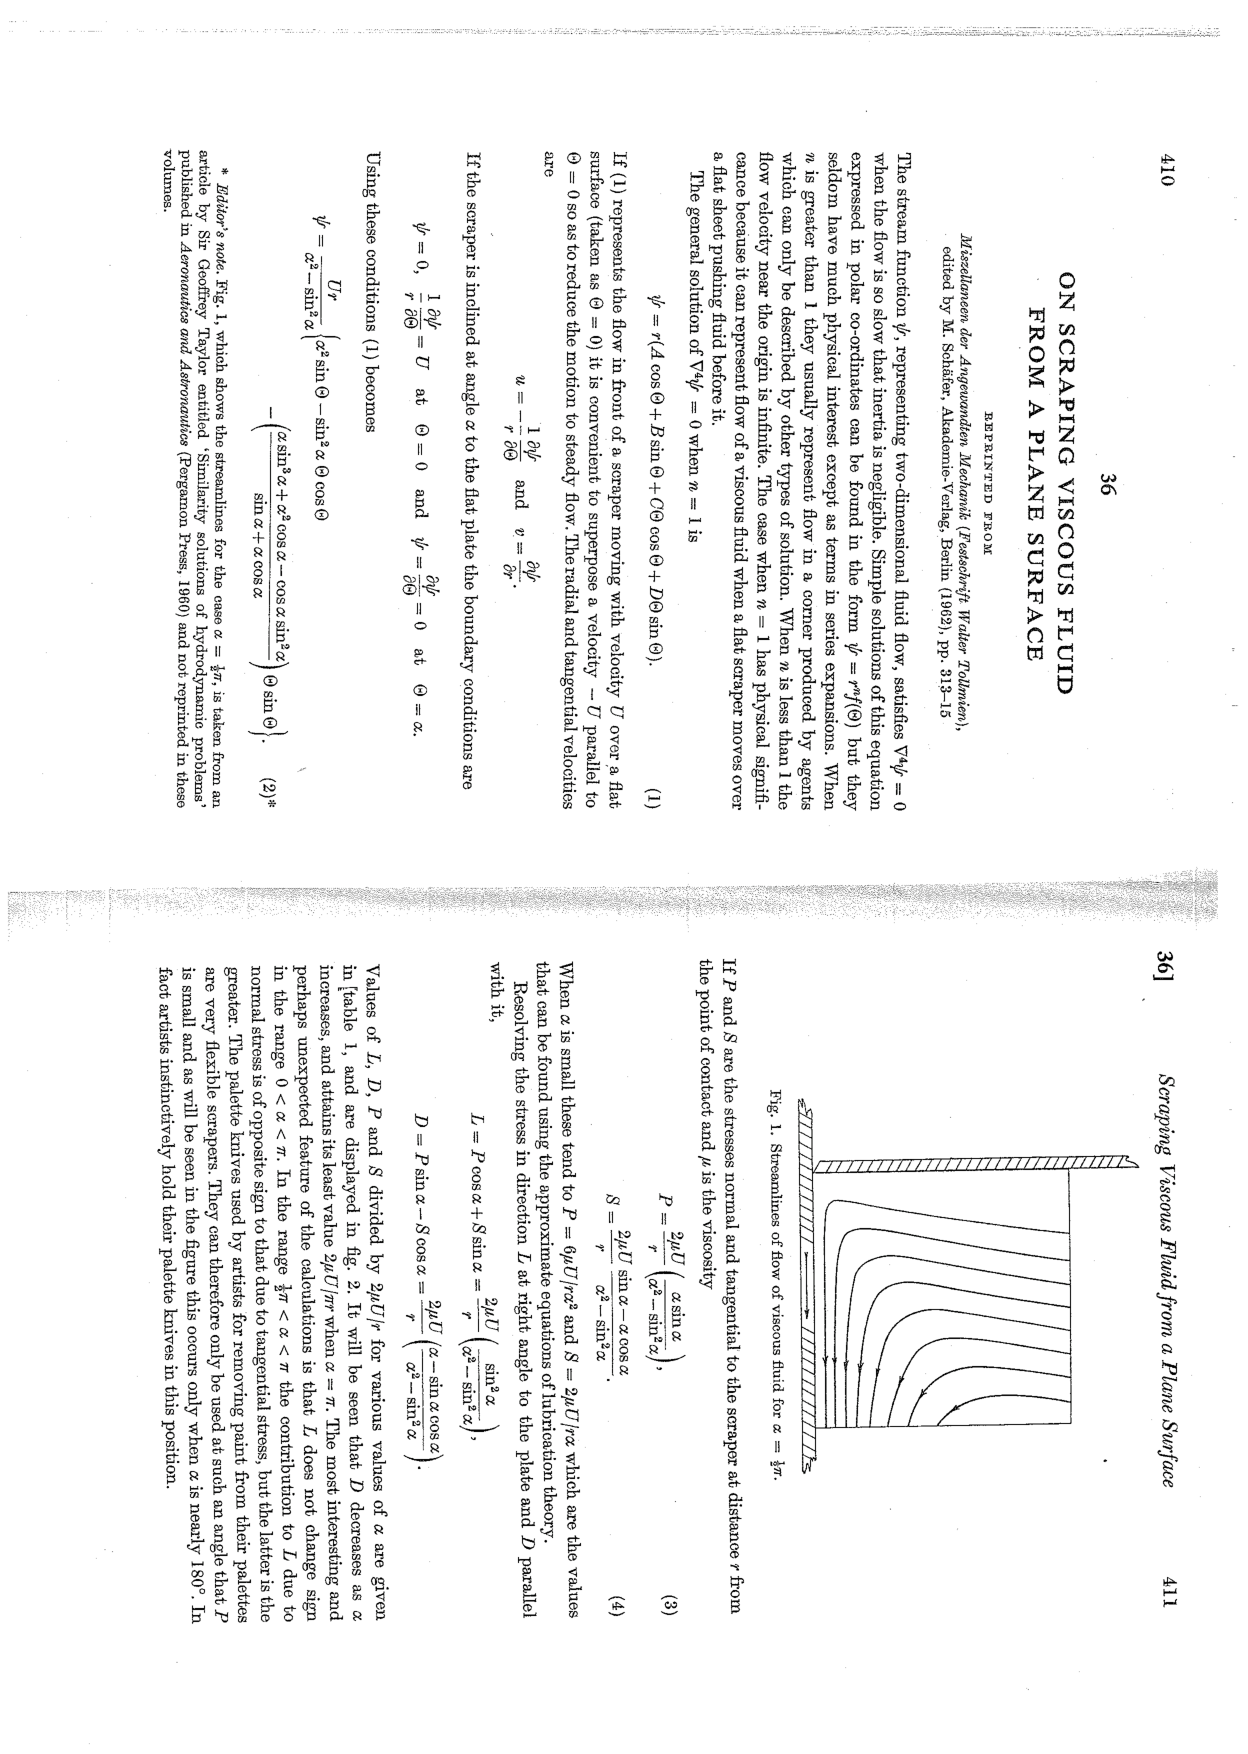
\includepdf[pages={1-2},rotate=90,landscape=true]{Taylor_scraping_viscous_fluid.pdf}
%\bibliographystyle{jfm}
%\bibliography{biblio_tuto}
\end{document}